\documentclass[conference]{IEEEtran}
\IEEEoverridecommandlockouts
% The preceding line is only needed to identify funding in the first footnote. If that is unneeded, please comment it out.
\usepackage{cite}
\usepackage{amsmath,amssymb,amsfonts}
\usepackage{algorithmic}
\usepackage{graphicx}
\usepackage{textcomp}
\usepackage{tikz}
\usepackage{tikzscale}
\usetikzlibrary{backgrounds,calc,decorations.pathreplacing,fit,matrix,patterns,positioning,shapes,shapes.multipart}
\def\BibTeX{{\rm B\kern-.05em{\sc i\kern-.025em b}\kern-.08em
    T\kern-.1667em\lower.7ex\hbox{E}\kern-.125emX}}
\begin{document}

\title{An Preliminary Investigation into Stateless Blockchain}

\author{
\IEEEauthorblockN{Yang Ji}
\IEEEauthorblockA{Dept. of Computer Science \\
ID: 56064832}
}

\maketitle


\section{Introduction}
Recent years have witnessed the prosperity of cryptocurrencies which seek for more efficient and secure financial
transactions through removing trusted third parties like escrows and banks~\cite{SongWP00}.
%
As their underlying technology, blockchain enables users to broadcast and confirm asynchronous transactions securely in an untrusted environment.
%
In order to achieve this, nodes in blockchain systems need to validate broadcasted transactions by querying the current system \textit{state}.
%
To be more specific, this state can be available by storing subsequent ordered blocks from the genesis block in local.

However, due to the ever-growing nature of the blockchain systems, the storage requirement is increasing linearly with the ledger length.
%
This restricted condition entails taking much storage space and time to download and maintain the entire history of blockchains.
%
For example, a new full node that wants to join in the Ethereum network and acquires the correct ledger \textit{state} needs to download 132.57 GB of data~\cite{Ethereumstorage} currently. 

As the emerging concerns on chain data size in the developer community, the concept of `stateless' blockchain has received considerable interests nowadays.
%
This concept is derived from a personal blog~\cite{delayed-txo-commitments}, which is proposed to avoid storing the whole state in an accumulative manner.
%
Unfortunately, realizing a blockchain system with lessened storage requirement is a quite difficult task due to many challenges.

For one thing, maintaining a public ledger in a decentralized system entails the duties of validating and broadcasting transaction on each node.
%
In order to check the validation of each transaction, nodes must store the current ledger \textit{state} that determines the ownership of existing assets.
%
For instance, the \textit{state} of Bitcoin is a data set of unspent transaction outputs (UTXOs). 
%
In order to check the validation of transactions, nodes should confirm that spent coin belongs to UTXO set locally.
%
In other words, nodes without storing UTXO set can't validate the incoming transactions.

For another thing, sharding or commitment schemes are viewed as effective methods to reduce the storage cost on each node.
%
In these ways, nodes could verify transactions by checking the membership proofs provided by issuers.
%
However, these solutions are actually at the cost of communication overhead across the system.
%
And high communication overhead would inevitably lead to the low scalability and throughput of the entire network, which is against the principles of cryptocurrencies.
%
How to leverage these tools to realize a cryptocurrency protocol is a challenging open question in blockchain community.

With these unresolved problems, I conduct an investigation into state-of-the-art solutions of stateless blockchain in this paper.
%
By categorizing existing literatures, I
%
I then pick up some important literatures and explain their algorithms in more detail.
%
By providing comprehensive evaluations for these methods, 

The rest of this paper is organized as follows: 


\begin{figure}[t]
  \centering
  \resizebox{0.7\linewidth}{!}{\begin{tikzpicture}[remember picture]
    \node (light-node){
        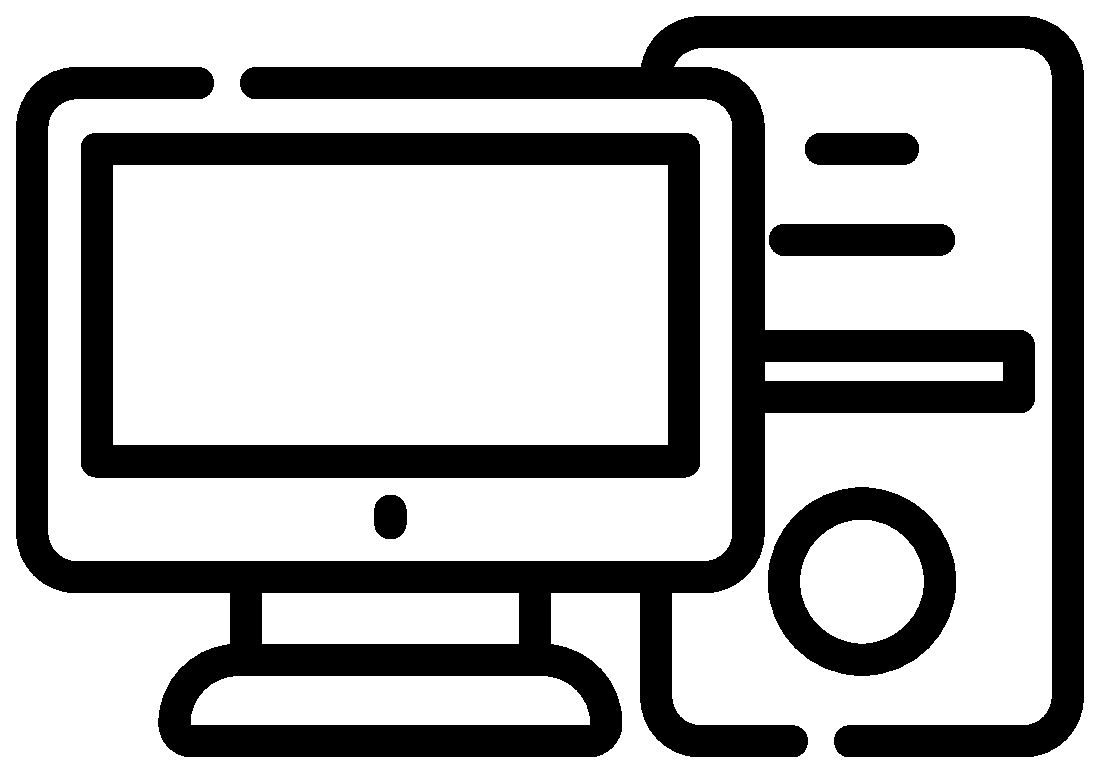
\includegraphics[scale = 0.05]{figs/icons/computer.eps}
    };
    \node[scale = 0.35,below=0cm of light-node] (light-label) {\textbf{Light Node}};

    \node (full-node) [matrix, below left = of light-node]{ 
        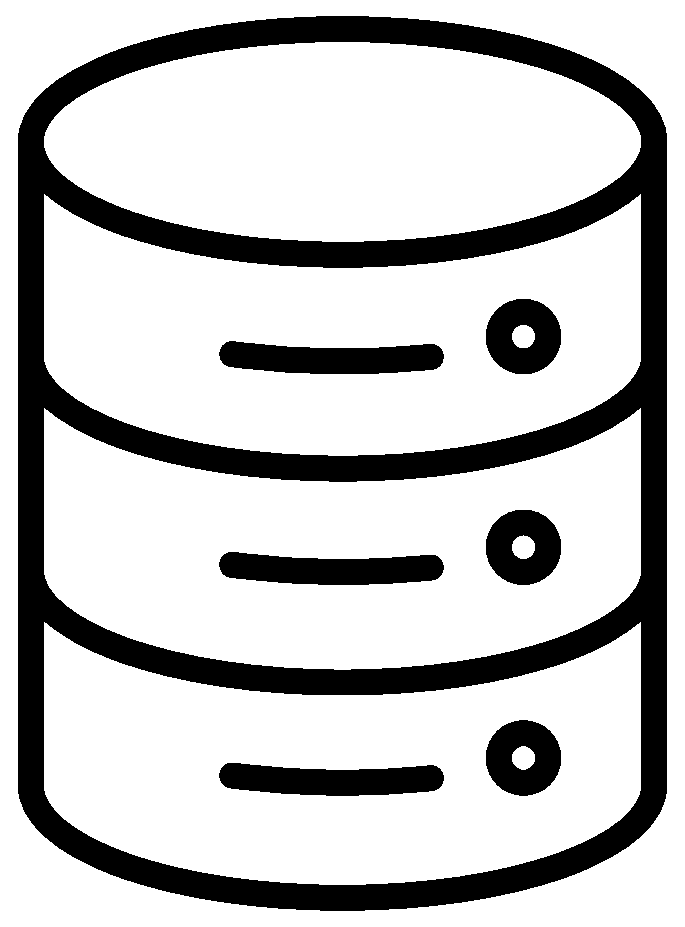
\includegraphics[scale = 0.05]{figs/icons/database.eps}
        \\
    };
    \node[scale = 0.35,below = 0cm of full-node,xshift=5ex] (full-label) {\textbf{Full Node}};

    \node (miner) [matrix, below right = 1.02cm and 0.5cm of light-node]{
        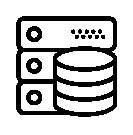
\includegraphics[scale = 0.45]{figs/icons/server.eps}
        \\
    };
    \node[scale = 0.35,below = 0cm of miner,xshift=6.5ex] (miner-label) {\textbf{Miner}};

    \draw [->] (-0.45,-0.05) -- (-1.3,-0.85) 
    node [above,midway,sloped,scale=0.3]
    {Info Request};

    \draw [<-] (-0.38,-0.17) -- (-1.15,-0.9) 
    node [below,midway,sloped,scale=0.3]
    {Answers \& Proof};

    \draw  (-1.15,-1.2) -- (1.2,-1.2);

    \draw [->] (0.45,-0.05) -- (1.35,-0.8) 
    node [above,midway,sloped,scale=0.3]
    {Info Request};

    \draw [<-] (0.42,-0.17) -- (1.22,-0.82) 
    node [below,midway,sloped,scale=0.3]
    {Answers \& Proof};
\end{tikzpicture}}
  \caption{System Architecture}\label{fig:model}
\end{figure}

\section{Application Setting}
\subsection{System Architecture}
In this subsection, I will briefly introduce the system architecture of current blockchains.
%
As shown in Figure, there exist three kinds of nodes with different functionalities in a classical blockchain network:
\textit{full nodes}, \textit{miners} and \textit{light nodes}.
%
To fulfill the security model, full nodes must download blocks originated from the first block all the way and validate them against consensus proof.
%
To be specific, a full node store all blocks including block headers and data records on the disk.
%
Miners are full nodes with high computational power, who could execute consensus protocol (e.g. hash puzzle in Bitcoin) and generate new blocks for money rewards.
%
Restricted in limited resources, a light node only needs to download block headers during the initial syncing process and then requests transactions from connected full nodes as needed.

\subsection{Stateless Blockchain}
In the current blockchain system, locally maintaining the validation state means quite cumbersome work. 
%
On one hand, this high storage requirement potentially fails those users who can't dedicate large storage space to join in the network.
%
More than that, increasing storage requirement might also reduce the incentives for running full nodes, which could lead to possible centralization of blockchains.
%
On the other hand, full nodes tend to leverage database (e.g. LevelDB in geth client) to manage the entire ledger \textit{state},
which causes expensive I/O costs and prolong the validation time.

Due to the above concerns, the blockchain community is eager for a well-designed protocol to tackle these issues by lessening or even removing local validation state.

%\begin{table}[h]
%\centering
%\caption{Comparison of encrypted search schemes.}
%\label{my-label}
%\begin{tabular}{|l|l|l|}
%\hline
%Scheme & Search Complexity & Index Size \\ \hline
%\cite{SongWP00}   & ...              & ...       \\ \hline
%...    & ...               & ...        \\ \hline
%\end{tabular}
%\end{table}



\section{Background on transaction validation in current blockchain systems}
In this part, I will take Ethereum as an example to untangle the intricacies in the data storage layer that exists in full nodes.
%
In Ethereum, developers have implemented many optimizations on the original data structure called Merkle Patricia Tries.
%
These data in local databases and on-chain block headers jointly contribute to the `World State' in blockchains.
%
What's more, the concept of `stateless' blockchain can be also applied into lightweight node. 
%
I will explain the details later.

\begin{figure}[!t]
  \centering
  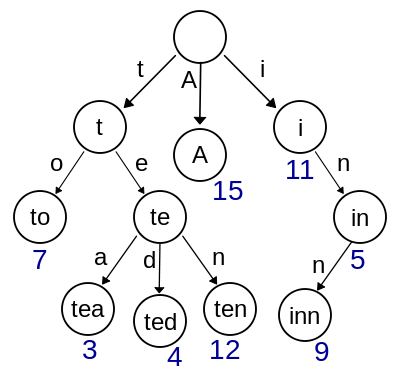
\includegraphics[width=2in]{figs/Trie.png}
  \caption{Trie Data Structure}
  \label{trie}
\end{figure}

\subsection{Data Storage in Full Node}
The core data structures which exist in Ethereum are made up of optimized Merkle Patricia Tries.
%
The term trie is derived from the word `Re{\textbf{tri}}eve' and the same as tree. 
%
Trie data structure, which is also called digital tree, radix tree and prefix tree, could be used to store the dynamic maps of key-value.  
%
We can efficiently traverse a branch of nodes in the trie with the reference to the corresponding keys.
%
For example, in Figure~\ref{trie}, the sequence of English alphabet is used to comprise the key. 
%
In the path of retrieving the value, the same sequences are grouped together to avoid massive of wasted space.

Many optimized implementations have been applied into the Ethereum's trie data structure in order to increase the search efficiency and performance.
%
In the Ethereum's official document, Merkle Patricia trie are defined as a cryptographically authenticated data structure that is used to store all bindings of key and value.
%
The hash function of each node, as I have mentioned in my first assignment before, could guarantee the data integrity and provide fast verification for users.
%
As for query processing, this unique data structure enables inserting, searching and deleting operations in the complexity of O(log(n)).
%
In engineering, some encoding schemes like Hex-Prefix encoding and Recursive Length Prefix (RLP) are also used for improving the query performance.
%
To conclude that, tries are enforced with cryptographic security by leveraging the hash function to reference each node.
%
And these tries could provide the efficient inserting, searching and deleting operations in local databases (Leveldb or Rocksdb).

\begin{figure}[!t]
  \centering
  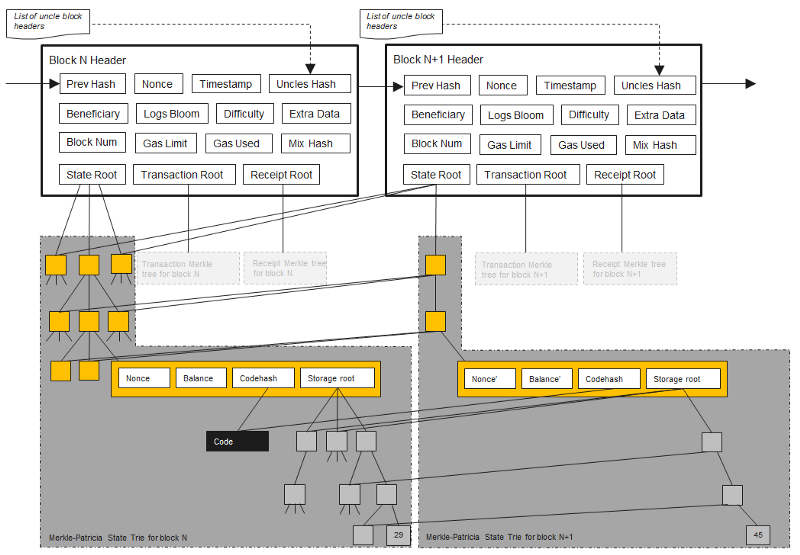
\includegraphics[width=\linewidth]{figs/Ethereum-tree.png}
  \caption{Ethereum Storage Layer}
  \label{e-trie}
\end{figure}

In order to maintain the state of the whole blockchain, Ethereum blocks contain four distinct trie data structures: (1)\textit{Receipt Tree} (2)\textit{State Tree} (3)\textit{Transaction Tree} (4)\textit{Storage Tree}.
%
As illustrated in Figure~\ref{e-trie}, The hash roots of first three merkle patricia tries are stored in the block headers in the form of Keccak 256-bit hash value. 
%
The hash root of \textit{Storage Tree} is included in \textit{State Tree} with its RLP encoded data records.

In more detail, \textit{Transaction Trie} is proposed to record transactions in the current block.
%
Thus, once the block is appended into the main chain, \textit{Transaction Trie} is also fixed and never updated.
%
Same as \textit{Transaction tree}, \textit{Receipt Tree} is used to record the outcome of transactions and never updated.
%
In Ethereum yellow paper\cite{Ethereumstorage}, \textit{Receipt Tree} could be used for zero-knowledge proofs or index and searches.
%
\textit{Receipt Tree} contains post-transaction state, cumulative gas used, logs and bloom filter created by the information of logs.
%
Different from the above trees, \textit{State Tree} records a key-value pair for each Ethereum account in an accumulative way.
%
\textit{State Tree} is actually only one global state tree which contains all past account information.
%
Thus, each time a miner generates a new block successfully, she also needs to update this global state correspondingly.
%
Because Ethereum leverages smart contract to achieve reliable computation in an untrusted environment, some extra space is needed to store these contract codes permanently.
%
Ethereum introduces contract accounts to manage these contracts and each contract account has a separate storage trie for that.

\subsection{Data Storage in Lightweight Node}
In practice, many devices with limited computing resources and storage space can't run as a full node.
%
Therefore, in Bitcoin white paper\cite{nakamoto2008bitcoin}, Satoshi Nakamoto puts forward a mechanism called simplified payment verification (SPV) to simplify transaction validation.
%
Through utilizing this mechanism, lightweight client only needs to download all the block headers during the syncing process.
%
Due to the lack of validation resources, lightweight node must query network nodes to download past blocks until she convinces that she has the correct ledger state.

In general, block headers contain enough information to assure that 
\begin{enumerate}
  \item Consensus proof (e.g. nonce) that is used to be against malicious provers.
  \item specific transactions in blocks.
  \item block depth used to convince the validation of transactions.
\end{enumerate}

It is worth nothing that block depth is totally opposite to block height and corresponds to the cumulative difficulty originated from the genesis block.
%
Once SPV client retrieves merkle branch and validates the existence of transaction in a block, she can only rely on the consensus mechanism for the security assurance. 


\section{Research Directions of Stateless Blockchain}
%
The concept of `stateless blockchain' is derived from the Peter Todd's blog post~\cite{Tod,MMR} because full nodes in blockchain might validate new appending transactions without storing all past blocks originated from the genesis block.
%
Originally, nodes verify the correctness of new transactions by querying local databases that keep all state and history in blockchains.
%
To address this issue radically, nodes could only need to store a short commitment to the current state instead of storing the whole ledger state.
%
Thus, the issuer of transactions needs to add an assets proof for validation. 
%
In this way, individual nodes only need to store the a set of own UTXO/accounts along with their proofs.
%
These proofs are used to prove the membership or non-membership of any elements in a set.
%
The na\"ive accumulator is Merkle Hash Tree.
%
There are also other authenticated data structures that have specific optimizations.
%
Except for hash-based tree, vector commitment also provides the functionality of position binding.
%
But these two methods have their own advantages and disadvantages.
%
I will analyse and compare these two methods later.
%
Since the concept of `stateless blockchain' is quite new in related field, there are few literature studies on it.
%
Hence, I will explain the state-of-the-art solutions comprehensively and list the trade-offs therein.


\subsection{Hash-based Accumulator}
\textbf{Goals.} The final purpose is to reduce the storage requirement for newly joining the network or validating the transactions.
%
Since the protocol and mechanism of transaction validation has changed over, original authenticated data structure (Merkle Hash Tree in Bitcoin and Merkle Patricia tree in Ethereum) should be designed again. 

\textbf{Design challenges.} 
Designing new authenticated index structures should consider the following aspects:

\begin{itemize}
  \item \textbf{Short membership/non-membership proofs.} 
  Since stateless blockchain needs an additional field (Merkle tree branch), overlong proof size might increase communication overhead inevitably.
  High communication overhead might lead to network latency and low the entire network throughput totally.
  \item \textbf{Support more efficient updating and inserting.}
  As a cryptocurrency, blockchain updates its global state frequently. Bitcoin generates a new block every 10 $\sim$ 12 minutes and in Ethereum generating a new block only needs 10 $\sim$ 15 seconds.
  Frequent updating operations on ledger state needs users to update local information to the newest.
  \item \textbf{Support any participant to update membership proofs.}
  As mentioned before, pending transactions need a uncertain time to be confirmed (Or never be confirmed due to low incentive or double-spend problem).
  However, the commitment of Merkle hash tree updates frequently, and as a result, the initial witness is not valid any more.
  To address this issue, we need to allow every miner to update witness freely.
\end{itemize}

\textbf{Related work.}
Peter Todd proposed Merkle Mountain Tree (MMR)~\cite{Tod} used for distributed time-stamping services atop Bitcoin in 2013. 
%
The data structure of MMR allows individual nodes to append new data without reconstructing the tree from scratch and keep a balanced state all the time.
%
As is shown in Figure~\ref{e-trie}, each time we append a subtree with new block headers, we only need to modify only a few nodes in the original tree and still keep the proof size in log\(n\).
%
Another advantage of this authenticated data structure is that only a tiny modifications need be done on the base of current blockchain systems.
%
However, this design lacks enough theoretical support including complexity analysis for updating and experimental result.

Based on MMR, Todd then put forward TXO (Transaction Output) commitment as opposed to UTXO commitment.
%
Once an transaction output is appended into the TXO MMR, this output is never removed.
%
To an extreme extent, individual nodes could only rely on TXO MMR, and as a result, eliminate the issue of unlimited growth of UTXO set.
%
What's more, nodes only need to append new data instead of updating TXO set frequently.
%
However, the complexity log\(n\) could increase bandwidth overhead inevitably.
%
Hence, individual nodes also need to maintain UTXO set for recent transactions and TXO set is only needed when very old coins are spent.
%
There are also some optimizations on UTXO and TXO sets.

Even though, there are still some unresolved problems in this proposal as follows:

\begin{itemize}
  \item \textbf{Incentive for storing less information.} 
        Incentive mechanism in current blockchain systems actually requires miners to store all information in local database (even in RAM for high competitiveness).
        In my opinion, transforming all past UTXO history to TXO MMR can't alleviate this issue at all since the growth of TXO set is also unlimited (even faster).
        If a miner doesn't store TXO set locally, she might lose competitiveness against other miners.
        In other words, competitive nodes would choose 
  \item \textbf{Incentive}
\end{itemize}



%
In this paper\cite{luuflyclient}, the authors adopt merkle mountain tree commitment and propose a probabilistic protocol only for lightweight client.
%


\subsection{Vector Commitment}

\textbf{Goals.} The description goes here.


\textbf{Design challenges.} The description goes here.

\textbf{Related work.} The description goes here.





\section{Conclusion}

The conclusion goes here.


\bibliographystyle{IEEEtran}
\bibliography{references}


\end{document}
